\documentclass[12pt, twoside]{article}
\input{../preamble}
\usepackage{pgfplots}
\usepgfplotslibrary{fillbetween}
\pgfplotsset{compat=1.16}

\fancyhead[LE]{\thepage}
\fancyhead[RO]{Name: \hspace{4cm} \,\\ \hspace{2.9cm} \,}
\fancyhead[LO]{La Scuola d'Italia / Dr.\ Huson / IB Math: Calculus \\* 1 April 2026}

\begin{document}
\subsubsection*{5.11 Classwork: Trigonometric Functions, Identities, \& Integration
(no calculator)}

\begin{enumerate}

\item The graph of $f(x) = \sin x$ for $0 \leq x \leq 2\pi$ is shown.
The regions $R_1$ and $R_2$ are shaded.

\begin{center}
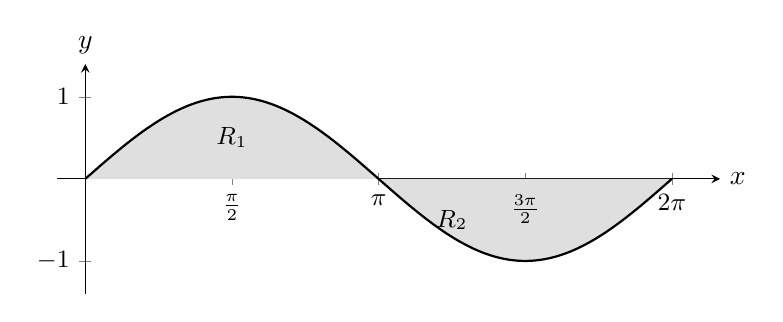
\begin{tikzpicture}
\begin{axis}[
    width=10cm, height=4.5cm,
    axis lines=middle,
    xlabel={$x$}, ylabel={$y$},
    xmin=-0.3, xmax=6.8,
    ymin=-1.4, ymax=1.4,
    xtick={1.5708, 3.1416, 4.7124, 6.2832},
    xticklabels={$\frac{\pi}{2}$, $\pi$, $\frac{3\pi}{2}$, $2\pi$},
    ytick={-1, 1},
    tick label style={font=\small},
    every axis x label/.style={at={(ticklabel* cs:1)}, anchor=west},
    every axis y label/.style={at={(ticklabel* cs:1)}, anchor=south},
]
\addplot[name path=F, thick, domain=0:6.2832, samples=200] {sin(deg(x))};
\addplot[name path=zero, draw=none, domain=0:6.2832] {0};
\addplot[gray!25] fill between[of=F and zero, soft clip={domain=0:3.1416}];
\addplot[gray!25] fill between[of=F and zero, soft clip={domain=3.1416:6.2832}];
\node at (axis cs:1.5708, 0.5) {\small $R_1$};
\node at (axis cs:3.927, -0.5) {\small $R_2$};
\end{axis}
\end{tikzpicture}
\end{center}

\begin{enumerate}
\item[(a)] Find $\displaystyle\int_0^{\pi} \sin x \,\mathrm{d}x$. \hfill [3]
\vspace{4cm}
\item[(b)] Write down the value of
$\displaystyle\int_{\pi}^{2\pi} \sin x \,\mathrm{d}x$. \hfill [1]
\vspace{1cm}
\item[(c)] Explain why $\displaystyle\int_0^{2\pi} \sin x \,\mathrm{d}x = 0$,
even though the shaded regions clearly have area. \hfill [2]
\vspace{1.5cm}
\item[(d)] Find the total area enclosed between the graph of $f$ and the $x$-axis
from $x = 0$ to $x = 2\pi$. \hfill [1]
\end{enumerate}
\vspace{0.5cm}

\newpage
\item The graph of $f(x) = \cos^2 x$ for $0 \leq x \leq \pi$ is shown.
The shaded region $R$ is bounded by the graph and the $x$-axis
from $x = 0$ to $x = \dfrac{\pi}{4}$.

\begin{center}
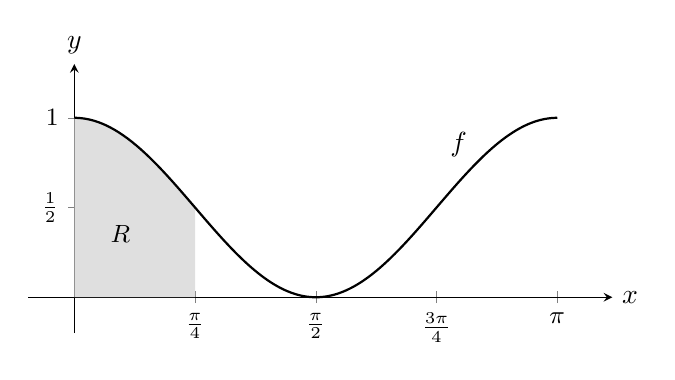
\begin{tikzpicture}
\begin{axis}[
    width=9cm, height=5cm,
    axis lines=middle,
    xlabel={$x$}, ylabel={$y$},
    xmin=-0.3, xmax=3.5,
    ymin=-0.2, ymax=1.3,
    xtick={0.7854, 1.5708, 2.3562, 3.1416},
    xticklabels={$\frac{\pi}{4}$, $\frac{\pi}{2}$, $\frac{3\pi}{4}$, $\pi$},
    ytick={0.5, 1},
    yticklabels={$\frac{1}{2}$, $1$},
    tick label style={font=\small},
    every axis x label/.style={at={(ticklabel* cs:1)}, anchor=west},
    every axis y label/.style={at={(ticklabel* cs:1)}, anchor=south},
]
\addplot[name path=F, thick, domain=0:3.1416, samples=200] {(cos(deg(x)))^2};
\addplot[name path=zero, draw=none, domain=0:3.1416] {0};
\addplot[gray!25] fill between[of=F and zero, soft clip={domain=0:0.7854}];
\node at (axis cs:0.3, 0.35) {\small $R$};
\node at (axis cs:2.5, 0.85) {$f$};
\end{axis}
\end{tikzpicture}
\end{center}

\begin{enumerate}
\item[(a)] Using the identity $\cos 2x = 2\cos^2 x - 1$, show that
$\cos^2 x = \dfrac{1}{2}(1 + \cos 2x)$. \hfill [2]
\vspace{5cm}
\item[(b)] Hence find $\displaystyle\int \cos^2 x \,\mathrm{d}x$. \hfill [3]
\vspace{4cm}
\item[(c)] Find the exact area of the shaded region $R$. \hfill [3]
\end{enumerate}


\newpage
\item The graphs of $g(x) = \sin^2 x$ (solid) and $h(x) = \cos^2 x$ (dashed) are
shown for $0 \leq x \leq \pi$. The dotted line is $y = \frac{1}{2}$.
The shaded region is bounded by $g$ and the $x$-axis.

\begin{center}
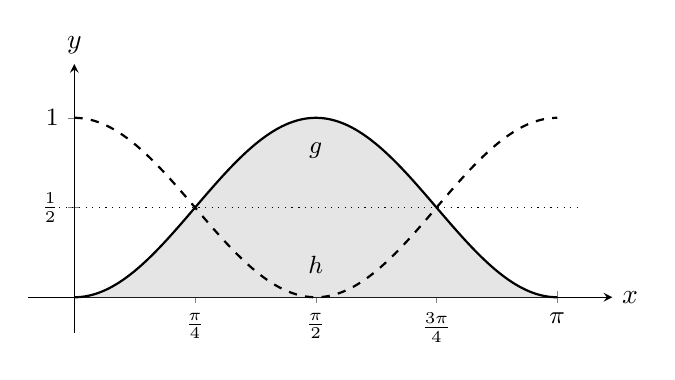
\begin{tikzpicture}
\begin{axis}[
    width=9cm, height=5cm,
    axis lines=middle,
    xlabel={$x$}, ylabel={$y$},
    xmin=-0.3, xmax=3.5,
    ymin=-0.2, ymax=1.3,
    xtick={0.7854, 1.5708, 2.3562, 3.1416},
    xticklabels={$\frac{\pi}{4}$, $\frac{\pi}{2}$, $\frac{3\pi}{4}$, $\pi$},
    ytick={0.5, 1},
    yticklabels={$\frac{1}{2}$, $1$},
    tick label style={font=\small},
    every axis x label/.style={at={(ticklabel* cs:1)}, anchor=west},
    every axis y label/.style={at={(ticklabel* cs:1)}, anchor=south},
]
\addplot[name path=S, thick, domain=0:3.1416, samples=200] {(sin(deg(x)))^2};
\addplot[thick, dashed, domain=0:3.1416, samples=200] {(cos(deg(x)))^2};
\addplot[thin, dotted, domain=-0.1:3.3] {0.5};
\addplot[name path=zero, draw=none, domain=0:3.1416] {0};
\addplot[gray!20] fill between[of=S and zero];
\node at (axis cs:1.5708, 0.82) {\small $g$};
\node at (axis cs:1.5708, 0.18) {\small $h$};
\end{axis}
\end{tikzpicture}
\end{center}

\begin{enumerate}
\item[(a)] The graphs intersect at $x = \dfrac{\pi}{4}$.
Verify this by evaluating $\sin^2\!\dfrac{\pi}{4}$ and
$\cos^2\!\dfrac{\pi}{4}$. \hfill [2]
\vspace{3cm}
\item[(b)] Show that $\sin^2 x = \dfrac{1}{2}(1 - \cos 2x)$. \hfill [2]
\vspace{4cm}
\item[(c)] Find $\displaystyle\int_0^{\pi} \sin^2 x \,\mathrm{d}x$. \hfill [4]
\vspace{4cm}
\item[(d)] Without further integration, find
$\displaystyle\int_0^{\pi} \cos^2 x \,\mathrm{d}x$.
Justify your answer. \hfill [2]
\end{enumerate}

\newpage
\item The function $f$ is defined by $f(x) = 4\sin x \cos x$
for $0 \leq x \leq \pi$.
The graph of $f$ is shown. The shaded region $R_1$ is bounded by the graph
and the $x$-axis from $x = 0$ to $x = \dfrac{\pi}{2}$.

\begin{center}
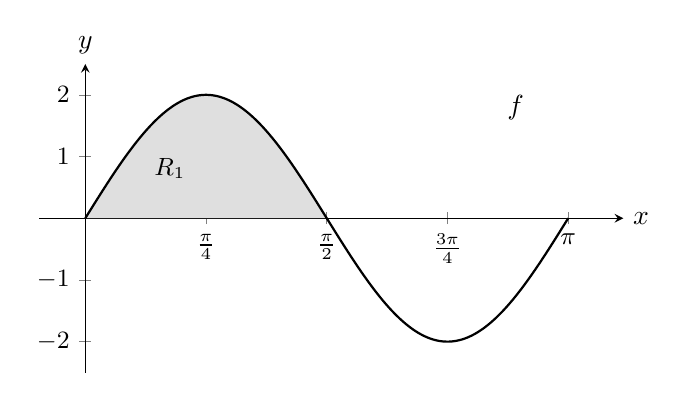
\begin{tikzpicture}
\begin{axis}[
    width=9cm, height=5.5cm,
    axis lines=middle,
    xlabel={$x$}, ylabel={$y$},
    xmin=-0.3, xmax=3.5,
    ymin=-2.5, ymax=2.5,
    xtick={0.7854, 1.5708, 2.3562, 3.1416},
    xticklabels={$\frac{\pi}{4}$, $\frac{\pi}{2}$, $\frac{3\pi}{4}$, $\pi$},
    ytick={-2, -1, 1, 2},
    tick label style={font=\small},
    every axis x label/.style={at={(ticklabel* cs:1)}, anchor=west},
    every axis y label/.style={at={(ticklabel* cs:1)}, anchor=south},
]
\addplot[name path=F, thick, domain=0:3.1416, samples=200]
    {4*sin(deg(x))*cos(deg(x))};
\addplot[name path=zero, draw=none, domain=0:3.1416] {0};
\addplot[gray!25] fill between[of=F and zero, soft clip={domain=0:1.5708}];
\node at (axis cs:0.55, 0.8) {\small $R_1$};
\node at (axis cs:2.8, 1.8) {$f$};
\end{axis}
\end{tikzpicture}
\end{center}

\begin{enumerate}
\item[(a)] Using the identity $\sin 2x = 2\sin x \cos x$,
show that $f(x) = 2\sin 2x$. \hfill [2]
\vspace{3cm}
\item[(b)] Write down the period of $f$. \hfill [1]
\vspace{0.5cm}
\item[(c)] Find the exact area of $R_1$. \hfill [4]
\vspace{3cm}
\item[(d)] Find the total area enclosed between the graph of $f$ and the $x$-axis
from $x = 0$ to $x = \pi$. Give a reason. \hfill [2]
\vspace{1.2cm}
\item[(e)] Find $f'(x)$ and hence find the $x$-coordinate where $f$ has its
maximum value on $\left[0, \dfrac{\pi}{2}\right]$. \hfill [2]
\end{enumerate}

\end{enumerate}
\end{document}
